\documentclass[table]{beamer}
%[]中可以使用draft、handout、screen、transparency、trancompress、compress等参数

%指定beamer的模式与主题
\mode<presentation>
{
  \usetheme{Madrid}
%\usetheme{Boadilla}
%\usecolortheme{default}
%\usecolortheme{orchid}
%\usecolortheme{whale}
%\usefonttheme{professionalfonts}
}

%\usetheme{Madrid}
%这里还可以选择别的主题:Bergen, Boadilla, Madrid, AnnArbor, CambridgeUS, Pittsburgh, Rochester, Warsaw, ...
%有导航栏的Antibes, JuanLesPins, Montpellier, ...
%有内容的Berkeley, PaloAlto, Goettingen, Marburg, Hannover, ...
%有最小导航栏的Berlin, Ilmenau, Dresden, Darmstadt, Frankfurt, Singapore, Szeged, ...
%有章和节表单的Copenhagen, Luebeck, Malmoe, Warsaw, ...

%\usecolortheme{default}
%设置内部颜色主题(这些主题一般改变block里的颜色);这个主题一般选择动物来命名
%这里还可以选择别的颜色主题,如默认的和有特别目的的颜色主题default,structure,sidebartab,全颜色主题albatross,beetle,crane,dove,fly,seagull,wolverine,beaver

%\usecolortheme{orchid}
%设置外部颜色主题(这些主题一般改变title里的颜色);这个主题一般选择植物来命名
%这里还可以选择别的颜色主题,如默认的和有特别目的的颜色主题lily,orchid,rose

%\usecolortheme{whale}
%设置字体主题;这个主题一般选择海洋动物来命名
%这里还可以选择别的颜色主题,如默认的和有特别目的的颜色主题whale,seahorse,dolphin

%\usefonttheme{professionalfonts}
%类似的还可以定义structurebold,structuresmallcapsserif,professionalfonts


% 控制 beamer 的风格,可以根据自己的爱好修改
%\usepackage{beamerthemesplit} %使用 split 风格
%\usepackage{beamerthemeshadow} %使用 shadow 风格
%\usepackage[width=2cm,dark,tab]{beamerthemesidebar}

%插入音标
\usepackage{tipa}
\AtBeginDocument{
  \renewcommand\textipa{\fontencoding{T3}\selectfont}
}
\AtBeginDocument{
  \renewcommand\textipa[2][r]{{\fontfamily{cm#1}\tipaencoding #2}}
}
\renewenvironment{IPA}[1][r]
 {\fontfamily{cm#1}\tipaencoding}
 {}

% 设定英文字体
%\usepackage{fontspec}
\usepackage[no-math]{fontspec}
\setmainfont{Times New Roman}
\setsansfont{Arial}
\setmonofont{Courier New}

% 设定中文字体
\usepackage[BoldFont,SlantFont,CJKchecksingle,CJKnumber]{xeCJK}
%\setCJKmainfont[BoldFont={Adobe Heiti Std},ItalicFont={Adobe Kaiti Std}]{Adobe Song Std}
\setCJKmainfont[BoldFont={Adobe Heiti Std},ItalicFont={Adobe Kaiti Std}]{WenQuanYi Micro Hei}
\setCJKsansfont{Adobe Heiti Std}
\setCJKmonofont{Adobe Fangsong Std}
\punctstyle{hangmobanjiao}

\defaultfontfeatures{Mapping=tex-text}
\usepackage{xunicode}
\usepackage{xltxtra}

\XeTeXlinebreaklocale "zh"
\XeTeXlinebreakskip = 0pt plus 1pt minus 0.1pt

\usepackage{setspace}
\usepackage{colortbl,xcolor}
\usepackage{hyperref}
%\hypersetup{xetex,bookmarksnumbered=true,bookmarksopen=true,pdfborder=1,breaklinks,colorlinks,linkcolor=blue,filecolor=black,urlcolor=cyan,citecolor=green}
\hypersetup{xetex,bookmarksnumbered=true,bookmarksopen=true,pdfborder=1,breaklinks,colorlinks,linkcolor=cyan,filecolor=black,urlcolor=blue,citecolor=green}

% 插入图片
\usepackage{graphicx}
\graphicspath{{figures/}}
% 图文混排
\usepackage{picins}
\usepackage{floatflt}

% 可能用到的包
\usepackage{amsmath,amssymb}
%插入多媒体
%\usepackage{media9}
%\usepackage{movie15}
\usepackage{multimedia}
\usepackage{multicol}
\usepackage{multirow}

% 定义一些自选的模板,包括背景、图标、导航条和页脚等,修改要慎重
% 设置背景渐变由10%的红变成10%的结构颜色
%\beamertemplateshadingbackground{red!10}{structure!10}
%\beamertemplatesolidbackgroundcolor{white!90!blue}
% 使所有隐藏的文本完全透明、动态,而且动态的范围很小
\beamertemplatetransparentcovereddynamic
% 使itemize环境中变成小球,这是一种视觉效果
\beamertemplateballitem
% 为所有已编号的部分设置一个章节目录,并且编号显示成小球
\beamertemplatenumberedballsectiontoc
% 将每一页的要素的要素名设成加粗字体
\beamertemplateboldpartpage

% item逐步显示时,使已经出现的item、正在显示的item、将要出现的item呈现不同颜色
\def\hilite<#1>{
 \temporal<#1>{\color{gray}}{\color{blue}}
    {\color{blue!25}}
}

\renewcommand{\today}{\number\year 年 \number\month 月 \number\day 日}

%五角星
\usepackage{MnSymbol}

%去除图表标题中的figure等
\usepackage{caption}
\captionsetup{labelformat=empty,labelsep=none}

\usepackage{tabu}
\usepackage{multirow}
%表格自动换行
\usepackage{tabularx} 

% 千分号
%\usepackage{textcomp}

%罗马数字
\makeatletter
\newcommand{\rmnum}[1]{\romannumeral #1}
\newcommand{\Rmnum}[1]{\expandafter\@slowromancap\romannumeral #1@}
\makeatother

%分栏
\usepackage{multicol}

%\usepackage{enumitem}
%\usepackage{enumerate}

%键盘
\usepackage{keystroke}

%插入源代码
\usepackage{listings}
\lstset{
  language=bash,                  % 程序语言名称:TeX, Perl, R, sh, bash, Awk
  basicstyle=\normalsize\tt,      %\tt指monospace字体族,程序源代码使用此族字体表示更加美观
  numbers=left,                   % 行号位置(左侧)
  numberstyle=\small,             % 行号字体的字号
  stepnumber=1,                   % 行号的显示步长
  numbersep=5pt,                  % 行号与代码间距
  backgroundcolor=\color{white},  % 背景色;需要 \usepackage{color}
  showspaces=false,               % 不显示空格
  showstringspaces=false,         % 不显示代码字符串中的空格标记
  showtabs=false,                 % 不显示 TAB
  tabsize=4, 
  frame=shadowbox,                % 把代码用带有阴影的框圈起来
  captionpos=b,                   % 标题位置
  breaklines=true,                % 对过长的代码自动断行
  breakatwhitespace=false,        % 断行只在空格处
  extendedchars=false,            % 解决代码跨页时,章节标题,页眉等汉字不显示的问题
  %escapeinside={\%*}{*},         % 跳脱字符,添加注释,暂时离开 listings 
  %escapeinside=``,
  commentstyle=\color{red!50!green!50!blue!50}\tt,  %浅灰色的注释
  rulesepcolor=\color{red!20!green!20!blue!20},     %代码块边框为淡青色
  keywordstyle=\color{blue!70}\bfseries\tt,         %代码关键字的颜色为蓝色,粗体
  identifierstyle=\tt,
  stringstyle=\tt,                % 代码字符串的特殊格式
  keepspaces=true,
  breakindent=1em,
  %breakindent=22pt,
  %breakindent=4em,
  breakautoindent=true,
  flexiblecolumns=true,
  aboveskip=1em,                  %代码块边框
  xleftmargin=2em,
  xrightmargin=2em
}

%\setbeamercolor{alerted text}{fg=magenta}
\setbeamercolor{bgcolor}{fg=yellow,bg=cyan}
%\setbeamercolor{itemize/enumerate body}{fg=green}

\begin{document}

%\includeonlyframes{current}

\logo{
\includegraphics[height=0.08\textwidth]{tijmu.png}}

% 在每个Section前都会加入的Frame
\AtBeginSection[]
{
  \begin{frame}<beamer>
    %\frametitle{Outline}
    \frametitle{教学提纲}
    \setcounter{tocdepth}{3}
    \begin{multicols}{2}
      \tableofcontents[currentsection,currentsubsection]
      %\tableofcontents[currentsection]
    \end{multicols}
  \end{frame}
}
% 在每个Subsection前都会加入的Frame
\AtBeginSubsection[]
{
  \begin{frame}<beamer>
%%\begin{frame}<handout:0>
%% handout:0 表示只在手稿中出现
    \frametitle{教学提纲}
    \setcounter{tocdepth}{3}
    \begin{multicols}{2}
    \tableofcontents[currentsection,currentsubsection]
    \end{multicols}
%% 显示在目录中加亮的当前章节
  \end{frame}
}

% 为当前幻灯片设置背景
%{
%\usebackgroundtemplate{
%\vbox to \paperheight{\vfil\hbox to
%\paperwidth{\hfil
\includegraphics[width=2in]{tijmu_charcoal.png}\hfil}\vfil}
%}
\begin{frame}[plain]
  \begin{center}
    {\Huge Linux系统概论\\}
    \vspace{1cm}
    {\LARGE 天津医科大学\\}
    %\vspace{0.2cm}
    {\LARGE 生物医学工程与技术学院\\}
    \vspace{1cm}
    {\large 2017-2018学年下学期(春)\\ 2016级生信班}
  \end{center}
\end{frame}
%}



%\includeonlyframes{current}

\begin{frame}
  \frametitle{课堂纪律}
  \begin{alertblock}{不迟到早退、不缺勤走神}
  约束不明,申令不熟,将之罪也;既已明而不如法者,吏士之罪也。
  \end{alertblock}
  \pause
  %\begin{itemize}[<+-|alert@+>]
  \begin{itemize}[<+->]
    \item 只有正式上课前的请假有效
    \item 提前5分钟到教室,严禁迟到
    \item 上课期间手机关机或调成震动
    \item 上课期间离开教室先举手示意
    \item 课上有疑问的话先举手后提问
    \item 上课期间严禁交头接耳,大声喧哗
    \item 随机点名,缺勤扣分如下:1、3、6
    \item 缺勤三次或三次以上者,平时成绩为0
  \end{itemize}
\end{frame}

\begin{frame}
  \frametitle{自我介绍}
    \begin{description}
      \item[姓\qquad 名]伊现富(Yi Xianfu)
      \item[本\qquad 科]山东大学
      \item[硕\qquad 博]中国科学院
      \item[工作邮箱]\alert{yixfbio@gmail.com}
      \item[生活邮箱]yixf1986@gmail.com
      \item[手\qquad 机]\alert{156\ 2061\ 0763}
      \item[个人博客]\textcolor{gray}{http://yixf.name}
      \item[网络昵称]yixf, Yixf
    \end{description}
\end{frame}

% \begin{frame}
%   \frametitle{邮箱网盘}
%     \begin{enumerate}
%       \item 126邮箱
%         \begin{itemize}
%           \item 账号:bioinfo\_TIJMU@126.com
%           \item 密码:\texttt{C\&563f\&nzx!s}
%         \end{itemize}
%       \item \alert{百度云网盘}
%         \begin{itemize}
% 	  \item \alert{账号:bioinfo\_TIJMU@126.com}
% 	  \item \alert{密码:\texttt{566\&Us3Rp6\#C}}
%         \end{itemize}
%     \end{enumerate}
% \end{frame}

\begin{frame}
  \frametitle{授课规律}
  \begin{block}{每次课}
    \begin{itemize}
      %\item 课前5分钟播放相关视频
      \item 课前5~10分钟播放相关视频
      \item 课堂中不点名,但随机提问
      \item 提问重点回顾上节课的知识点
      %\item 授课内容以讲义为主、幻灯片为辅
      \item 授课内容以幻灯片为主、教材为辅
      %\item 讲授需要掌握的知识点和必备的技能
      %\item 讲义中给出参考资料与课外阅读材料
      %\item 幻灯片图多字少,以讲解为主
      \item 幻灯片图表多文字少,以讲解为主
      \item 开始有回顾和引言,最后有总结和答疑
    \end{itemize}
  \end{block}
  \pause
  \begin{block}{每一章}
    \begin{itemize}
      \item 复习思考题:知识点与技能
      \item 共享幻灯片、视频等所有授课资料
    \end{itemize}
  \end{block}
\end{frame}

\begin{frame}
  \frametitle{思考题}
  \begin{block}{问题}
  %\begin{enumerate}[<+-|alert@+>]
  \begin{enumerate}[<+->]
    \item 与他人交流信息的方式有哪些?
    \item 与他人共享资料的方法有哪些?
    \item 从哪些方面可以提高密码的强健度?
    \item 如果方便安全地管理众多的密码?
  \end{enumerate}
  \end{block}
  \pause
  \begin{block}{提示}
    \begin{enumerate}
      \item 电话、短信/微信/易信、邮件、面谈……
      \item U盘、邮箱、网盘……
      \item 唯一、复杂、勤换……
      \item KeePassX、LastPass、KeeWeb……
    \end{enumerate}
  \end{block}
\end{frame}

\begin{frame}
\end{frame}

\begin{frame}
  \frametitle{Linux与生物信息学}
  \begin{description}
    \item[编程语言] 很多生物信息学软件以C源代码包的形式进行发布,需要编译安装后才能使用;Linux是用C写的
    \item[作业支持] 生物信息的主要工作是用软件和脚本处理生物数据,尤其是生物大数据;Linux稳定、开源、免费,是服务器操作系统的首选,对高性能和大数据的支持好,高性能集群和云平台大多基于Linux
    \item[软件工具] 一般的生物信息分析软件都是基于Linux开发的;Linux中的生物信息软件包和脚本丰富,命令丰富,shell可编程能力强,定制设计和开发容易
    \item[文本处理] 生物信息学数据大多以纯文本进行保存;Linux中开箱即用的文本处理命令丰富、易用、高效
    \item[岗位要求] 生物信息学工作者使用最多的平台就是Linux操作系统;Linux是应聘生物信息学岗位的必备技能之一(Perl/Python,R,……)
    \item[脑洞大开] 我自豪、我骄傲、我懒惰、我专业、……
  \end{description}
\end{frame}

\begin{frame}
  \frametitle{课程目标}
  \begin{block}{适用对象}
    \begin{itemize}
      \item Linux新手,对Linux感兴趣
      \item Linux菜鸟,扩充Linux知识
      \item 期望应用Linux的生物信息学工作者
    \end{itemize}
  \end{block}
  \pause
  \begin{block}{不适用对象}
    \begin{itemize}
      \item 学习并掌握Linux内核/系统的计算机基础(本课程以应用为主)
      \item 成为Linux高手(修行在个人;唯手熟尔;一万小时定律)
      \item 掌握Linux的所有内容(没有一个人可以做到这一点)
    \end{itemize}
  \end{block}
  \pause
  \begin{block}{课程目标}
    \begin{itemize}
      \item 掌握Linux的基本常识,并能够熟练使用Linux
      \item 能够将Linux应用到日常的生物信息学工作中
    \end{itemize}
  \end{block}
\end{frame}

\begin{frame}
  \frametitle{可能的疑问}
  \begin{block}{两个问题}
  \begin{enumerate}
    \item \textcolor{gray}{【你的疑问】}课程是“Linux系统概论”,教材却是《Unix入门经典》。写错了?
    \item \textcolor{gray}{【我的疑问】}对于Linux,你是闻所未闻,还是“日用而不知”?
  \end{enumerate}
\end{block}
  \pause
  \begin{block}{简单的回答}
  \begin{enumerate}
    \item Linux和Unix的区别:前者免费,后者收费
    \item 口袋里的手机,搜索、网购背后的服务器,……
  \end{enumerate}
\end{block}
\end{frame}

\begin{frame}
  \frametitle{新的视野}
  \begin{figure}
    \centering
    \visible<1->{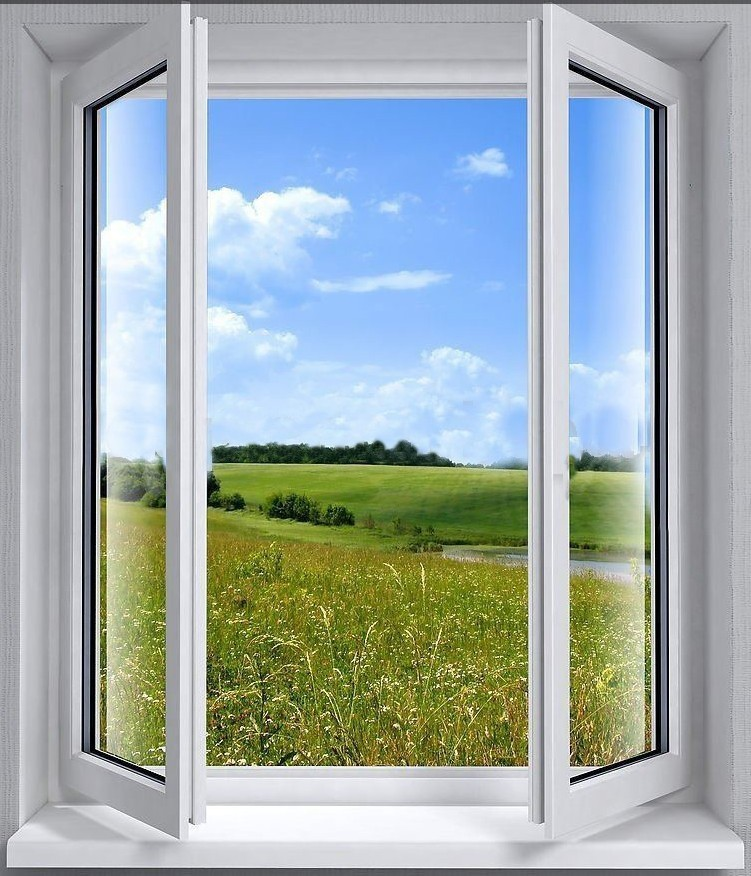
\includegraphics[width=5cm]{c0.windows.view.02.jpg}}
    \quad
    \visible<2->{
\includegraphics[width=5.4cm]{c0.linux.view.02.png}}
  \end{figure}
\end{frame}

\begin{frame}
  \frametitle{Linux的世界}
  \begin{figure}
    \centering
    %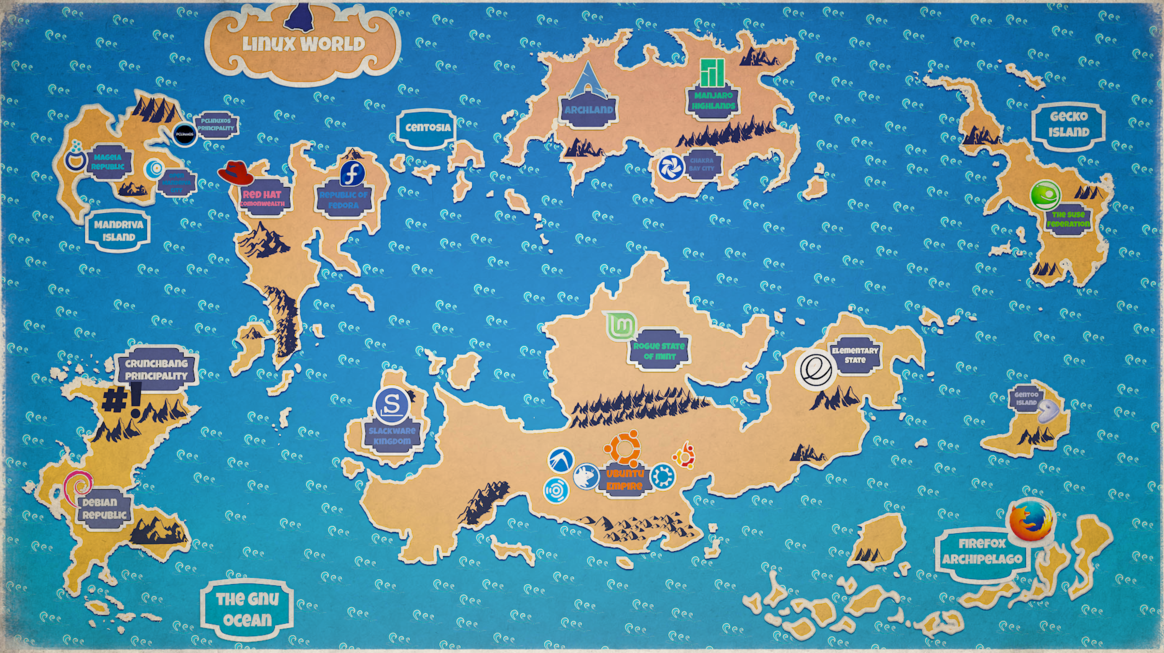
\includegraphics[width=12cm]{c0.linux.world.04.png}
    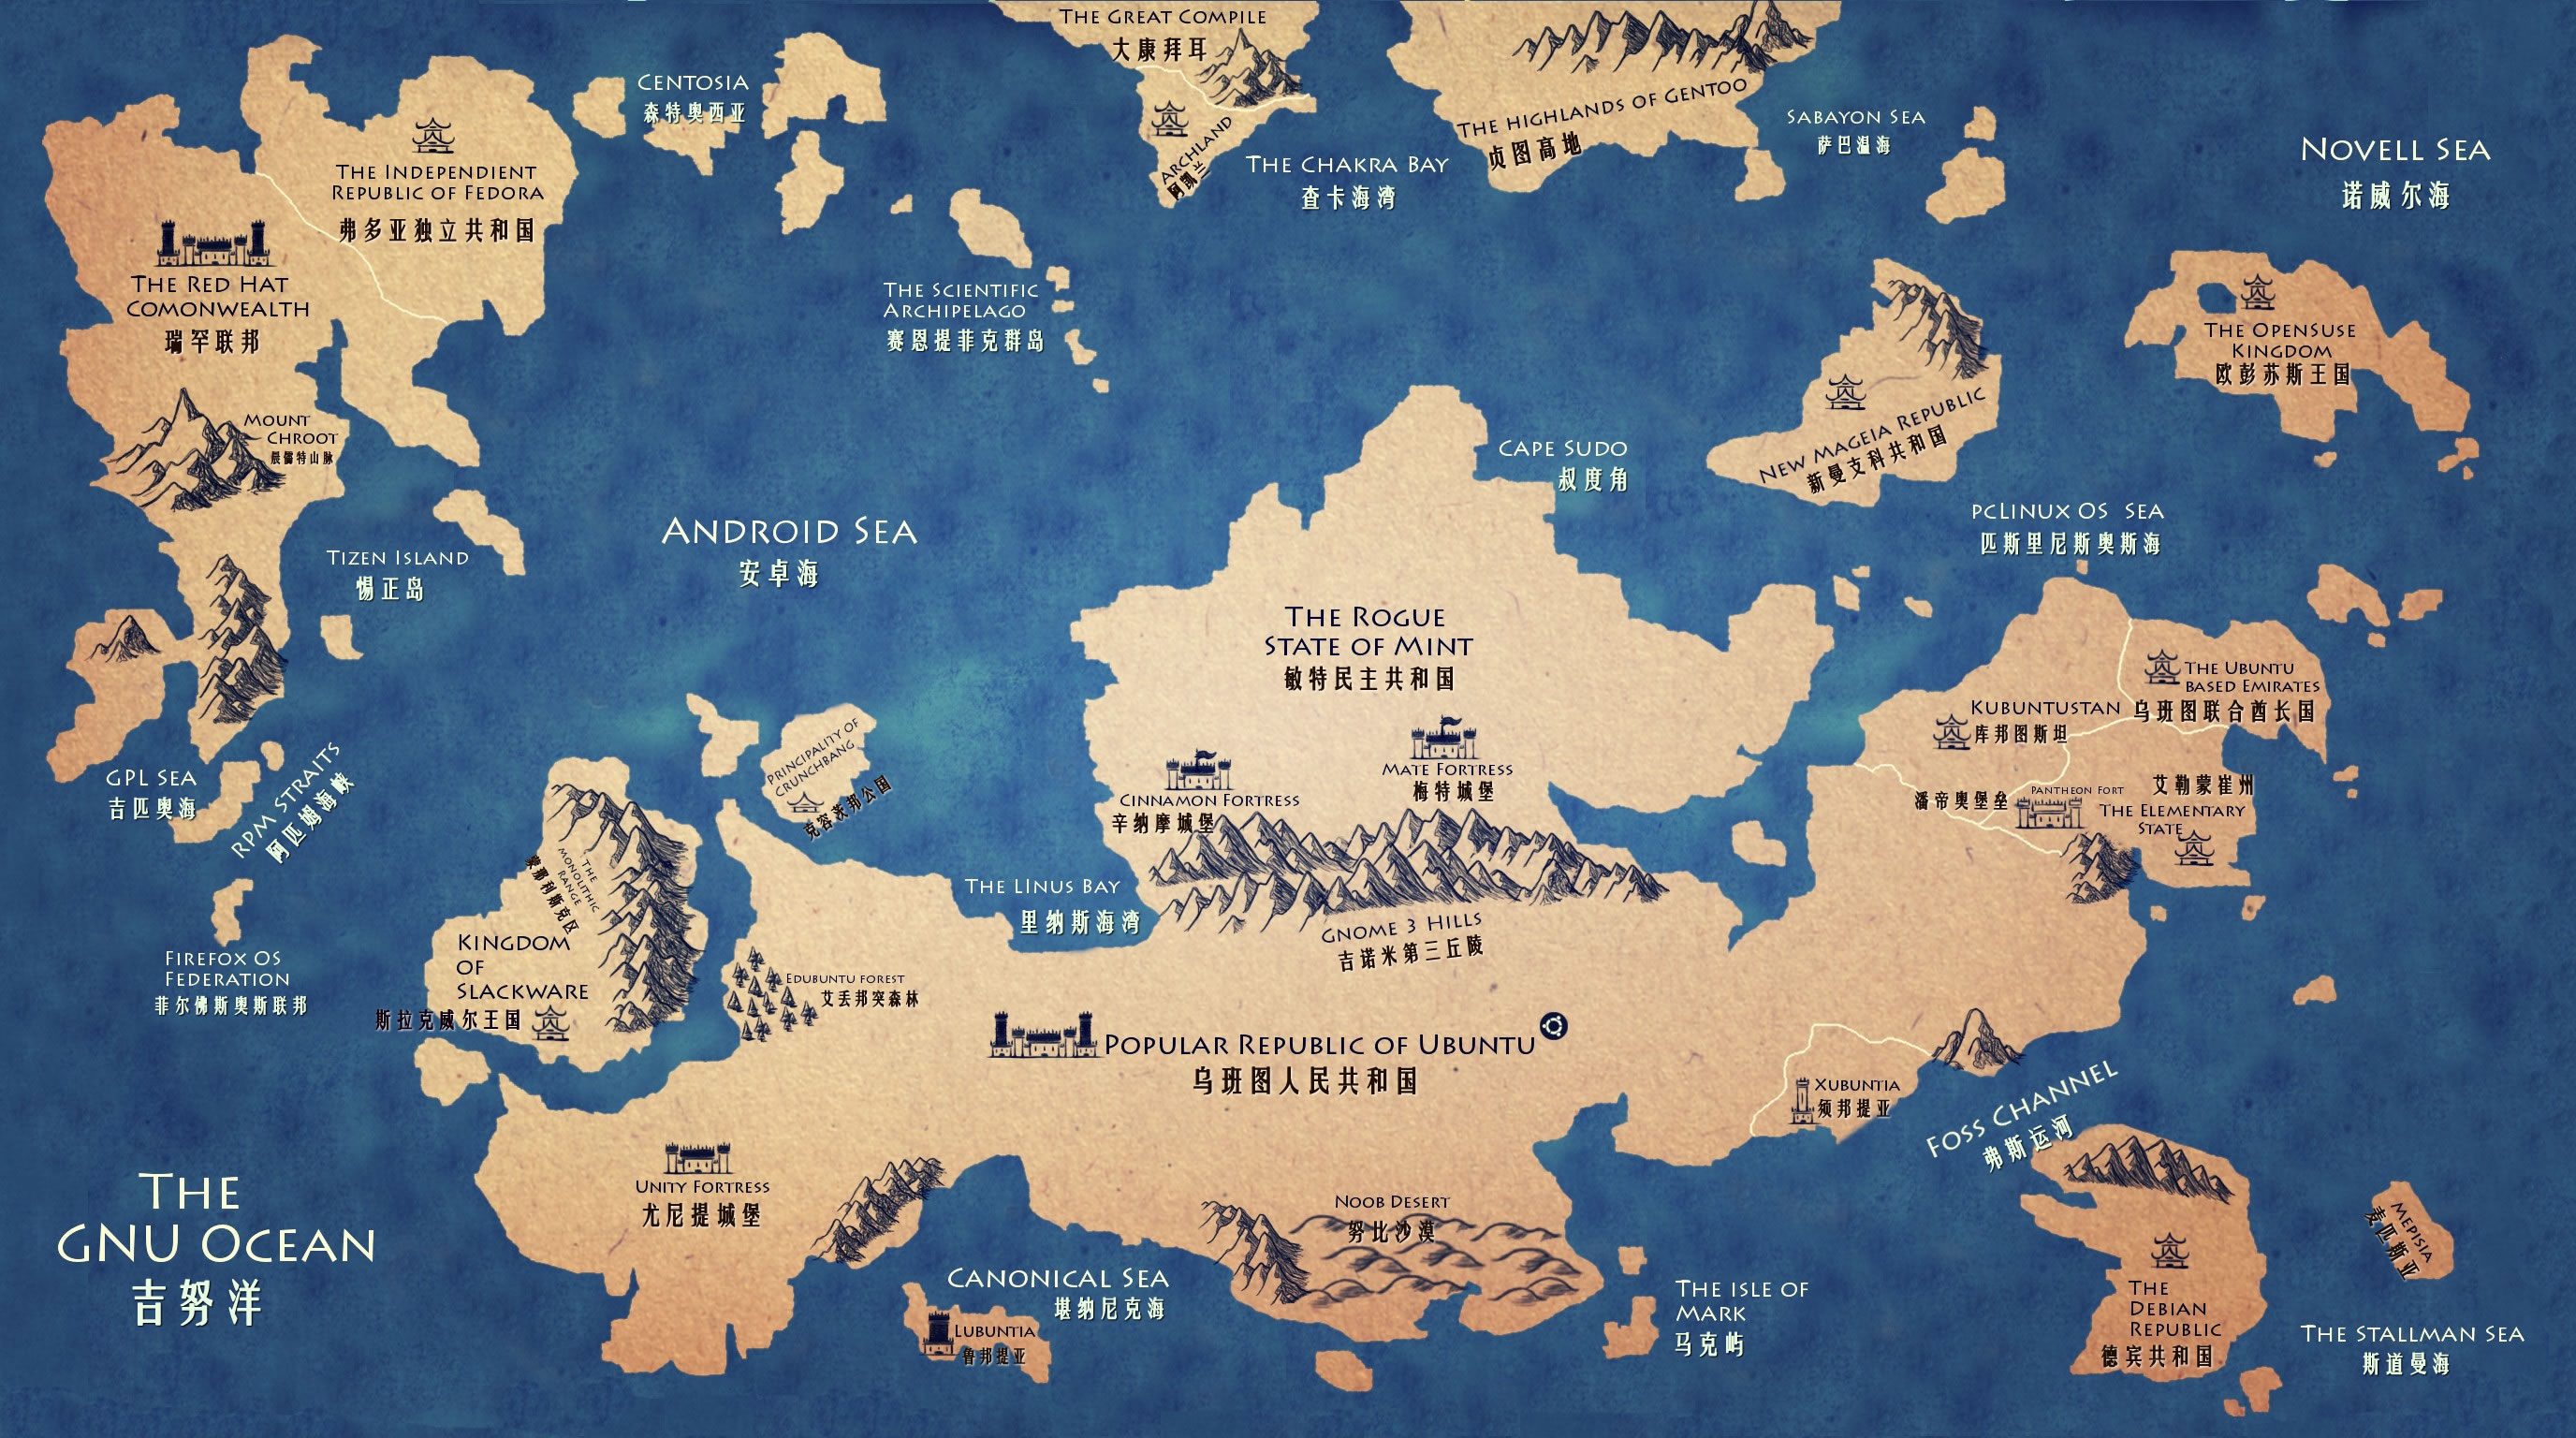
\includegraphics[width=12cm]{c0.linux.world.06.jpg}
  \end{figure}
\end{frame}

\begin{frame}
  \frametitle{授课教材}
  \begin{figure}
    \centering
    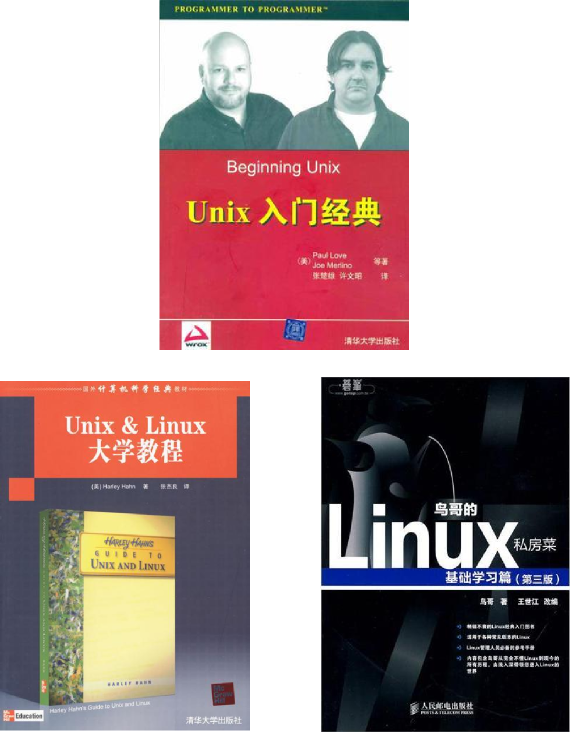
\includegraphics[width=6cm]{c0.books.png}
  \end{figure}
\end{frame}

\begin{frame}
  \frametitle{课程安排 | 理论课}
  \begin{center}
  \alert{前9周,每周三,上午前两节(8:00-9:50),西楼608}\\
  \vspace{0.2cm}
  {\footnotesize
  \textit{纯英文的幻灯片大部分摘抄自edX上的课程:\\ \href{https://www.edx.org/course/introduction-linux-linuxfoundationx-lfs101x-2}{LinuxFoundationX: LFS101x.2 Introduction to Linux}}
  }
  \end{center}
  \vspace{-0.5cm}
  \begin{table}
    \centering
    \rowcolors[]{1}{blue!20}{blue!10}
    \begin{tabular}{cllcc}
      \hline
      \rowcolor{blue!50}顺序 & 授课内容 & 教材章节 & 学时 & 日期\\
      \hline
      1 & Linux基础 & 第1、2章 & 2 & 3.2\\
      2 & 用户和组 & 第3章 & 2 & 3.9\\
      3 & 文件系统 & 第4章 & 2 & 3.16\\
      4 & Linux命令 & 第6章 & 2 & 3.23\\
      5 & 高级Linux命令 & 第8、9章 & 2 & 3.30\\
      6 & 软件安装 & 第19章 & 2 & 4.6\\
      7 & vi/Vim编辑器 & 第7章 & 2 & 4.13\\
      8 & shell脚本编程(上) & 第13、14章 & 2 & 4.20\\
      9 & shell脚本编程(下) & 第13、14章 & 2 & 4.27\\
      %9 & Perl语言简介 & 第17章 & 2 & 7.07\\
      \hline
    \end{tabular}
  \end{table}
\end{frame}

\begin{frame}
  \frametitle{课程安排 | 实验课}
  \begin{center}
  \alert{前9周,每周三,下午前两节(13:30-15:20),教一楼304}\\
  \vspace{0.2cm}
  {\footnotesize
  \textit{部分实验内容摘抄自:\\ 《Linux基础及应用习题解析与实验指导》(谢蓉\ 编著,第二版,中国铁道出版社)}
  }
  \end{center}
  \vspace{-0.5cm}
  \begin{table}
    \centering
    \rowcolors[]{1}{blue!20}{blue!10}
    \begin{tabular}{cllcc}
      \hline
      \rowcolor{blue!50}顺序 & 实验内容 & 理论知识 & 学时 & 日期\\
      1 & 在虚拟机中安装Linux & Linux基础 & 2 & 3.2\\
      2 & Linux图形界面下的文件操作 & \textcolor{gray}{文件系统} & 2 & 3.9\\
      3 & Linux命令行下的文件操作 & 文件系统 & 2 & 3.16\\
      4 & Linux常用命令操作 & Linux命令 & 2 & 3.23\\
      5 & Linux高级命令操作 & 高级Linux命令 & 2 & 3.30\\
      6 & Linux中软件的安装 & 软件安装 & 2 & 4.6\\
      7 & Vim编辑器的使用 & vi/Vim编辑器 & 2 & 4.13\\
      8 & shell脚本的编写(上) & shell脚本编程(上) & 2 & 4.20\\
      9 & shell脚本的编写(下) & shell脚本编程(下) & 2 & 4.27\\
      %9 & Perl脚本的编写 & Perl语言简介 & 2 & 7.09\\
      \hline
    \end{tabular}
  \end{table}
\end{frame}

\begin{frame}
  \frametitle{考核方式}
  \begin{enumerate}
    \item 理论课:60\%
      \begin{enumerate}
        \item 平时表现:10\%
        \item 闭卷考试:50\%
      \end{enumerate}
    \item 实验课:40\%
      \begin{enumerate}
        \item 平时表现:20\%
        \item 实验报告:20\%
      \end{enumerate}
  \end{enumerate}
\end{frame}




\section*{Acknowledgements}
\begin{frame}
  \frametitle{Powered by}
  \begin{center}
    
\includegraphics[width=9cm]{power.png}
  \end{center}
\end{frame}

\end{document}

